\documentclass[12pt, twoside]{article}
\usepackage{jmlda}
\newcommand{\hdir}{.}
\usepackage[utf8]{inputenc}
\usepackage[english,russian]{babel}
\usepackage{graphicx}
\usepackage{hyperref}       % hyperlinks
\usepackage{url}            % simple URL typesetting
\usepackage{booktabs}       % professional-quality tables
\usepackage{amsfonts}       % blackboard math symbols
\usepackage{nicefrac}       % compact symbols for 1/2, etc.
\usepackage{microtype}
\usepackage{lipsum}
\usepackage{longtable}
\usepackage{graphicx}
\usepackage{subcaption}
\usepackage{float}
\usepackage{amsmath}
\usepackage{multirow}

\begin{document}

\title
    [Step detection via deep learning] % краткое название; не нужно, если полное название влезает в~колонтитул
    {Step detection via deep learning}
\author
    [А.\,В.~Филиппова] % список авторов (не более трех) для колонтитула; не нужен, если основной список влезает в колонтитул
    {А.\,В.~Филиппова, Т.~Гадаев, В.\,В.~Стрижов} % основной список авторов, выводимый в оглавление
    [А.\,В.~Филиппова$^1$, Т.~Гадаев$^1$, В.\,В.~Стрижов$^{1}$] % список авторов, выводимый в заголовок; не нужен, если он не отличается от основного
% \email
   % {islamov.ri@phystech.edu; grabovoy.av@phystech.edu;  strijov@ccas.ru}
%\thanks
%    {Работа выполнена при
%     %частичной
%     финансовой поддержке РФФИ, проекты \No\ \No 00-00-00000 и 00-00-00001.}
\organization
    {$^1$Московский физико-технический институт}
\abstract
    {В данной работе рассматривается задача предсказания траектории человека по показаниям аксселрометра и гироскопа, которые установлены в телефоне. Так как система отсчета, связанная с устройством, постоянно вращается и движется ускоренно относительно мировой системы, поставленная задача не является тривиальной. Существует много различных необучаемых алгоритмов для описания траектории человека. Минус этих алгоритмов в том, что модель не может подстраиваться под конкретную постановку задачи и учитывать детали (пол, возраст, особенность походки объекта). В данной работе предлагается нейросетевой подход для решения задачи, а также описываются полезные эвристики. 
    
    Наше исследование можно разделить на три логические части: проектирование устойчивых к ошибкам гироскопов кватернионов, прогнозирование изменения положения на фиксированном периоде с помощью различных нейронных сетей и применение идеи детекции шагов с целью улучшения показаний модели и уменьшения дрифта.
\bigskip
\noindent


\textbf{Ключевые слова}: \emph {аксселерометр и гироскоп; детекция шагов ;кватернионы; дрифт; нейросетевой подход; предсказание траектории}
}

\maketitle
\linenumbers

\section{Введение}

Задача точного определения положения смартфона в пространстве,и, как следствие, оценка местоположения объекта решается с высокой точностью на открытых площадках с использованием GPS ~\cite{mohamed1999adaptive}. Современные технологии демонстрируют отличные результаты при отклонении менее чем на несколько метров ~\cite{rahiman2013overview}. Однако у системы есть недостаток: она требует открытого пространства между устройством и спутником для передачи радиосигналов. В реальном мире нас часто окружают деревья, неровности ландшафта, высокие здания. Качество геолокации снижается из-за отражения радиоволн. Например, использование GPS для отслеживания траекторий внутри зданий практически бесполезно ~\cite{dedes2005indoor}. В этом случае используются методы, основанные на данных других датчиков. Наиболее распространенными датчиками IMU смартфона являются гироскоп, магнитометр и акселерометр. Основной проблемой такого подхода является накопление ошибок позиционирования из-за дрейфа, вызванного несовершенствами и шумом в датчиках (тут будет ссылка на статью моего куратора, которая пока не была опубликована). В данной работе предлагается по мимо методов, описанных в статье  (тут будет ссылка на статью моего куратора, которая пока не была опубликована) использовать детекцию шагов с целью улучшения показаний модели и уменьшения дрифта.

\section{Постановка задачи}

Задача состоит в том, чтобы найти суперпозицию функций, которые мы обозначим как $F_{\text{tr+st}}$, которая преобразует данные датчиков в оценку траектории, , которая будет близка к истиной, а также дает оценку вероятности совершения шага вдоль траетории в каждый момент времени.
\begin{equation}
    \label{eq:general_ps}
    \argmin\limits_{F_{\text{tr+st}}}\mathcal{L}\left(F_{\text{tr+st}}\left(\cal{A}, \cal{W}\right), \cal{T}, \cal{S}\right)
\end{equation}{}
\newpage
В качестве функции потерь предлагается использовать комбинированную функцию  $\mathcal{L}\left(F_{\text{tr}}\left(\cal{A}, \cal{W}\right), \cal{T}, \cal{S}\right) = \textbf{MSE}\left(F_{\text{tr}}\left(\cal{A}, \cal{W}\right), \cal{T}\right) + \textbf{BCElogloss}\left(F_{\text{st}}\left(\cal{A}, \cal{W}\right), \cal{S}\right)$.

Данная функция потерь позволяет обучить модель таким образом, чтобы для вещественных выходов модели решалась задача регрессии, для категориальных - классификации. 



\section{Данные}

В эксперементе мы использовали набор данных RuDaCop~\cite{bayev2019rudacop}. Данные состоят из $1200$ измерений траекторий для разных положений смартфона (в руке, в сумке, в кармане брюк). Для каждого объекта сняты показания аксселерометра, гироскопа, координаты человека в мировой системе отсчета, состояние правой и левой ног ($0$ - поднята, $1$ - на земле). При сборке данных соблюдены следующие требования:
\begin{enumerate}
    \item Траектории находятся на плоских горизонтальных поверхностях - нет лестниц или значительных изменений высоты ландшафта.
    \item Все траектории замкнуты. Это означает, что точка начала равна точке финиша. Участников попросили использовать маркер для отметки положения старта, что позволяет утверждать, что разница в исходном и финишном положениях не более $5$ см для каждой
ноги.
\item Участники только ходили, другого движения (прыжков/бега) не было.
\item Участники не были ограничены в скорости движения.

Пример показаний аксселерометра представлен на изображении $1$.

\end{enumerate}
\begin{figure}[!h]
\center{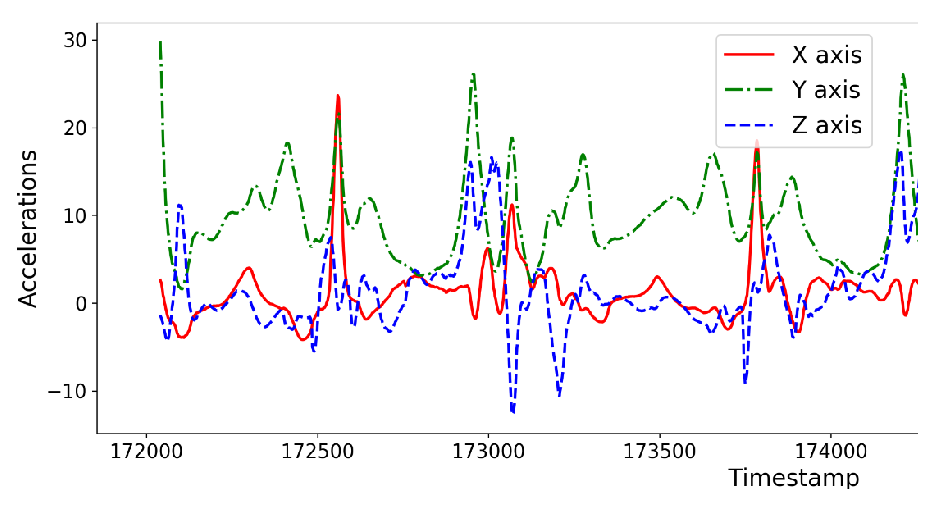
\includegraphics[scale=1]{acc_example.eps}}
\caption{Пример показаний аксселерометра}
\label{fig:image}
\end{figure}


\newpage

\section{Эксперимент}

\subsection{Архитектура}


Известно, что сверточные сети умеют хорошо выявлять локальную информацию в поданных объектах благодаря обучаемуму скрытому представлению (детекция изображений, сегментация изображений). Рекуррентные нейронные сети хорошо подходят для задач регрессии временных рядов, так как имеют способность "хранить" информацию. В данной статье предлагается использовать некоторую модификацию известной архитектуры ResNet, состоящей из чередования сверточных слоев, пулингов и residual block - техника позволяющая решать проблему "утекающего градиента". Наша архитектура ResNetLSTM - сетка, в которой последовательно соеденены ResNet и двухслойная LSTM. Архитектура сетки представлена на изображении $2.$



\begin{figure}[!h]
\center{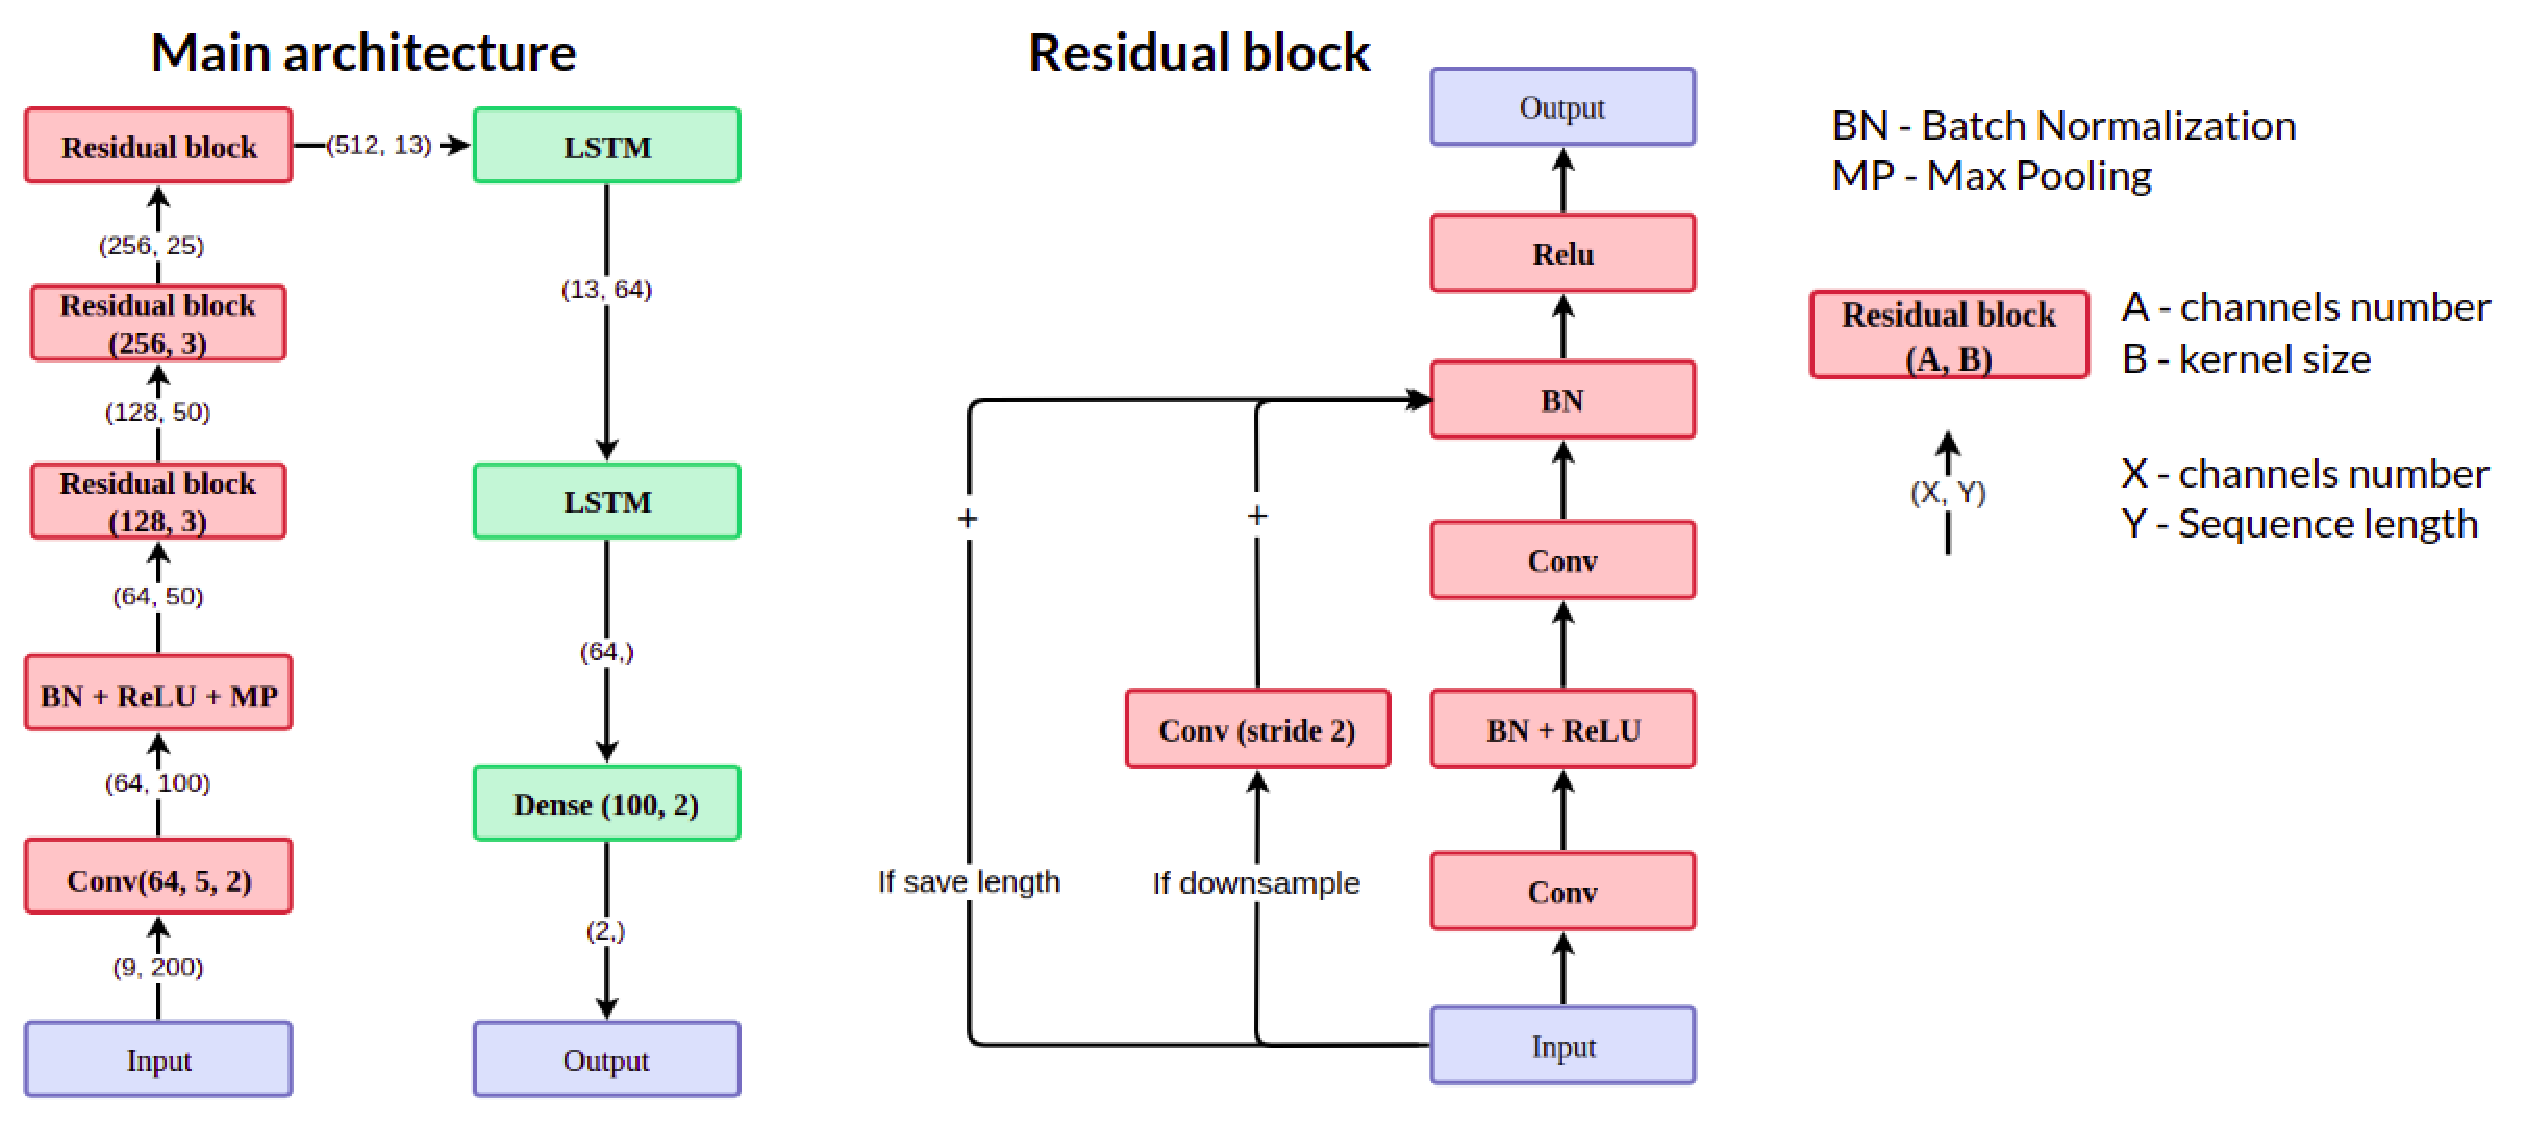
\includegraphics[scale=0.4]{architectures.eps}}
\caption{Cхема нейронной сети}
\label{fig:image}
\end{figure}


\subsection{Обучение}

На изображение $3$ представлен график лосса обучения и валидации сетки.


\begin{figure}[!h]
\center{\includegraphics[scale=0.5]{loss_on_train.jpg}}
\caption{Лосс во время обучения и валидации.}
\label{fig:image}
\end{figure}



\subsection{Результаты}

Пример предсказания.


\begin{figure}[!h]
\center{\includegraphics[scale=1]{prediction_example.eps}}
\caption{Пример предсказанной траектории.}
\label{fig:image}
\end{figure}
\newpage
\bibliographystyle{unsrt}
\bibliography{References}

\end{document}

